\section{Method}

\subsection{Root obervation}

To get to our method, start with the following observation:
Rigid bodies are treated as point masses in many cases because the precise shapes don't matter, but in the case of simulating their behavior moving through a medium field, they do matter.
To take an example---when a wooden plank falls into water, one side of it first touches the water, and the buoyancy force causes a torque, causing the plank to pitch (fig. \ref{fig:plank-falling-into-water-illustration}).
Had the plank taken as a simple point mass, the torque couldn't have been reflected;
also, the buoyancy force would have only taken effect after the center of mass of the plank passes the water surface.

\begin{figure}[h]
	\def\ih{1in}
	\centering
	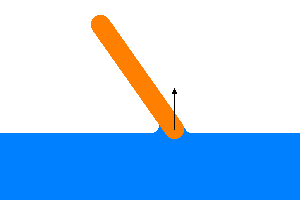
\includegraphics[height=\ih]{../Thesis/figures/stages-of-a-plank-falling-into-water/1.png}
	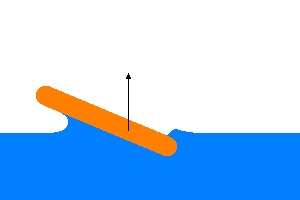
\includegraphics[height=\ih]{../Thesis/figures/stages-of-a-plank-falling-into-water/2.png}
	
\includegraphics[height=\ih]{../Thesis/figures/stages-of-a-plank-falling-into-water/3.png}
	\caption{The stages of a plank falling into water.}
	\label{fig:plank-falling-into-water-illustration}
\end{figure}

To ensure that the result is correct, the entire volume of the rigid body should be taken into consideration.
This sounds computational heavy, but luckily there is the \emph{divergence theorem} to simplify the case:
The integral of the divergence of a vector field ($\mathbf{F}$) over a volume ($V$) is equal to the flux of the field on the boundary of the volume (\ref{formula:divergence-theorem}).

\begin{equation}
	\iiint_{V}(\nabla\cdot\mathbf{F})\mathrm{d}V
	=
	\oiint_{\partial V}\left(\mathbf{F}\cdot\hat{\mathbf{n}}\right)\mathrm{d}\partial V
	.
	\label{formula:divergence-theorem}
\end{equation}

When applied on a fully or partially submerged solid object, this could lead to the famous \emph{Archimedes' principle};
but sadly, the derived principle only tells us how strong the buoyancy force is, but missing the torque information.
To gain the torque information, we need to manually break the integral into discretized elements to make sure every bit of information is included.

\subsection{Outline}

Comparing to discretizing and summing over the entire volume, it is obviously easier to just process the surface as directed by the right-hand side of (\ref{formula:divergence-theorem}).
The general steps of our method would be:
\begin{enumerate}
	\item Generate a random set of sample points over the surface of an target object.
	\item Calculate the small contributions of each point.
	\item Sum them up while preserving the torque information.
	\item Apply the summed effect on the target object.
\end{enumerate}
This process would be applied per target object (submerged in water) per frame.

\paragraph*{Step 1: Sample point generation}

This could be done by reading the object's mesh geometry data.
As common game engines all convert meshes into polygon soups of triangles, it is natural to pick a random triangle for each sample, and then pick a random point on it.

However, the chances of each triangle being picked will be the same using this approach, which means that smaller triangles would have the same amount of impact as larger triangles, contradicting the common physical sense.
The solution is to grant each sample point a weight that's proportional to the area of the triangle it's on, and the strength of their contributions will be scaled in step 3.

\paragraph*{Step 2: Local contribution calculation}

This step is pretty straight-forward---just calculate the water pressure based on the position and the normal direction of the point.

\paragraph*{Step 3: Summation}

First, the weights need to be applied on the contributions to make them proportional to the areas they represent, but the summation of these area also need to match with the actual surface area of the object.
The reason that the summed area might mismatch with the actual area is that there is no guarantee that each triangle face would be sampled at least once and only once in each round of sampling.
To fix this, multiply every contribution by an additional factor of $\frac{\text{actual area}}{\text{sum of sample areas}}$.

Then, to sum up the contributions, the point they take effect at must be taken into consideration for perserving the torque information.
By basic Newtonian physics, a force applied on a point on a rigid body could be transformed into an equivalent force applied on its center of mass plus a torque.
Formula (\ref{eq:force-transformation}) shows this transformation, in which $\mathbf r$ represents the delta position from the center of mass to the effect point.
\begin{equation}
	(\mathbf f,\mathbf r)_{\text{force on a point}}\mapsto(\mathbf f,\mathbf r\times\mathbf f)_{\text{force-torque tuple}}.
	\label{eq:force-transformation}
\end{equation}

Lastly, to add two force-torque pais together, simply perform vector addition member-wisely.

\paragraph*{Step 4: Applying}

The result from last step would be a single force-torque pair to be applied on the object.
Every mature game engine should provide physical interfaces of applying force and torque on the center of mass of rigid bodys.

\subsection{Adding frictional terms}

In real applications, one thing best not to be overlooked is the frictional terms.
They could ensure that the simulation of physical behaviors would eventually converge to a stable state due to energy loss.
Without them, it is easy to end up with numerical instability due to accumulated float-point arithmetic errors.

In the later experiment section of this article, three kinds of frictional terms are used:
\begin{itemize}
	\item Form drag, the repelling force caused by a surface moving with a relative velocity perpendicular to surrounding water, scaled by a factor $c_f$.
	\item Viscous drag, the dragging force caused by a surface moving with a relative velocity parallel to surrounding water, scaled by a factor $c_v$.
	\item Dissipation, forced ratio of kinetic energy loss per time.
				This is implemented outside of the scope of our method.
				It acts as a post-effect that is applied on all submerged bodies after all the physical updates are done in a frame.
\end{itemize}
Both drag forces are proportional to the half of the modulo of their corresponding relative velocities \cite{trouton1906coefficient}.

After adding these, the resulting formula for the water pressure on a sample point is given as (\ref{eq:resulting-pressure-formula}), where $v_{\perp}$ and $v_{\parallel}$ are the perpendicular and parallel relative velocities.:
\begin{equation}
	p=-\rho gh-\frac12c_f|v_{\perp}|^2-\frac12c_v|v_{\parallel}|^2.
	\label{eq:resulting-pressure-formula}
\end{equation}